%%%%%%%%%%%%%%%%%%%%%%%%%%
%%% author : Yamada. T %%%
%%% made for TH series %%%
%%%%%%%%%%%%%%%%%%%%%%%%%%

\documentclass[b5paper,10pt,fleqn] {ltjsarticle}

\usepackage[margin=10truemm]{geometry}

\usepackage{pict2e, graphicx}
\usepackage{tikz}
\usetikzlibrary{intersections,calc,arrows.meta}

\usepackage{amsmath, amssymb, amsthm}
\usepackage{ascmac}
\usepackage{comment}
\usepackage{empheq}
\usepackage[shortlabels,inline]{enumitem}
\usepackage{fancybox}
\usepackage{fancyhdr}
\usepackage{here}
\usepackage{lastpage}
\usepackage{listings, jvlisting}
\usepackage{fixdif}

\usepackage{stmaryrd}
\usepackage[listings]{tcolorbox}
%\usepackage{ascolorbox}
\usepackage{titlesec}
\usepackage{ulem}
\usepackage{url}
\usepackage{verbatim}
\usepackage{wrapfig}
\usepackage{xcolor}
\usepackage{luatexja-ruby}
\usepackage{varwidth}
\usepackage[version=3]{mhchem}
\usepackage{wrapfig}


\usepackage{physics2}
	\usephysicsmodule{ab}
	\usephysicsmodule{ab.braket}
	\usephysicsmodule{ab.legacy}
	%\usephysicsmodule{braket}
	\usephysicsmodule{diagmat}
	\usephysicsmodule{xmat}
	\usephysicsmodule{nabla.legacy}
	\usephysicsmodule{qtext.legacy}

\usepackage[ISO]{diffcoeff}
\difdef { f, s } { D }
{ op-symbol = \mathrm{D} }


\newcommand{\mctext}[1]{\mbox{\textcircled{\scriptsize{#1}}}}
\newcommand{\ctext}[1]{\textcircled{\scriptsize{#1}}}
\newcommand{\ds}{\displaystyle}
\newcommand{\comb}[2]{{}_{#1}\mathrm{C}_{#2}}
\newcommand{\hs}{\hspace}
\newcommand{\vs}{\vspace}
\newcommand{\emphvs}{\vspace{1em}\notag\\}
\newcommand{\ora}{\overrightarrow}
\newcommand{\ol}{\overline}
\newcommand{\oramr}[1]{\overrightarrow{\mathrm{#1}}}
\newcommand{\tri}{\triangle}
\newcommand{\mr}{\mathrm}
\newcommand{\mb}{\mathbb}
\newcommand{\mrvec}[1]{\overrightarrow{\mathrm{#1}}}
\newcommand{\itvec}{\overrightarrow}
\newcommand{\bs}{\boldsymbol}
\newcommand{\ra}{\rightarrow}
\newcommand{\Ra}{\Rightarrow}
\newcommand{\lra}{\longrightarrow}
\newcommand{\Lra}{\Longrightarrow}
\newcommand{\la}{\leftarrow}
\newcommand{\La}{\Leftarrow}
\newcommand{\lla}{\longleftarrow}
\newcommand{\Lla}{\Longleftarrow}
\newcommand{\lr}{\leftrightarrow}
\newcommand{\llr}{\longleftrightarrow}
\newcommand{\Llr}{\Longleftrightarrow}
\renewcommand{\deg}{{}^\circ}
\newcommand{\phbox}{\fbox{\phantom{1\hspace{2em}}}}
\newcommand{\boxnum}[1]{\fbox{\phantom{\hspace{1em}}({#1})\phantom{\hspace{1em}}}}
\newcommand{\boxkana}[1]{\fbox{\phantom{\hspace{1em}}{#1}\phantom{\hspace{1em}}}}
\newcommand{\boxkm}[2]{\fbox{\, {#1}\phantom{\hspace{0.2em}} \,  {#2}}}
\newcommand{\hzw}{\hspace{1\zw}}

\renewcommand{\baselinestretch}{1.25}
\parindent=1\zw


%TH3-29

\begin{document}
\noindent\fbox{NewTH4-5} [大阪大]

\begin{wrapfigure}{r}{7cm}
  \centering
  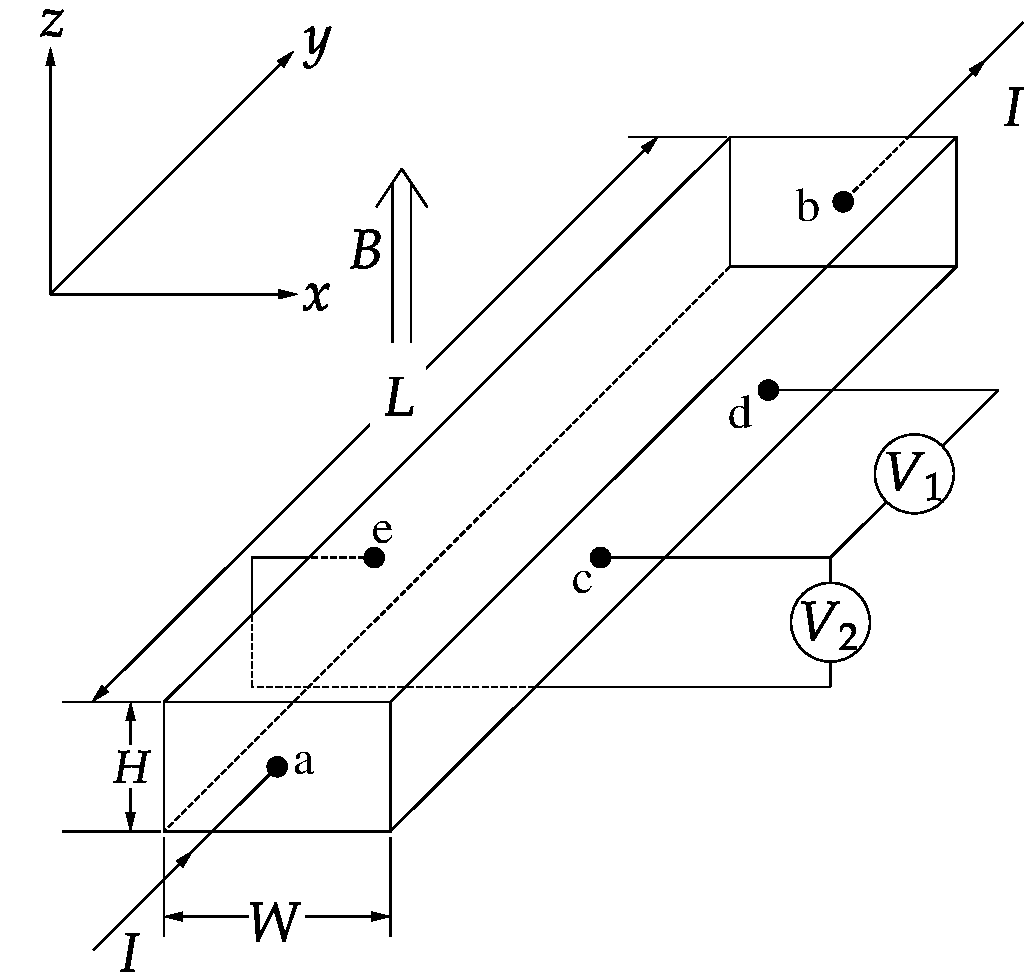
\includegraphics[width=7cm]{fig/fig_4_5_1.pdf}
  \caption{}
\end{wrapfigure}
次の文中の空欄に適切な答をそれぞれ記せ.

図1のように幅$W$〔m〕,高さ$H$〔m〕,長さ$L$〔m〕の直方体の形状をした半導体があり,その抵抗率を$\rho$\nobreak〔$\Omega \cdot \mr{m}$〕とする.
ただし,$L$は$W$,$H$に比べて十分に長いとする.

図1に示したように直方体の両端a,bに導線を付け,電流$I$〔A〕を$y$軸方向に流した.中心方向の直方体面上の点c,d,eの電位をそれぞれ$V_\mr{c}$〔V〕,$V_\mr{d}$\nobreak〔V〕,$V_\mr{e}$〔V〕としたときの電圧$V_1$〔V〕($= V_\mr{c} - V_\mr{d}$),$V_2$\nobreak〔V〕\nobreak($=V_\mr{c} - V_\mr{d}$)を測定した.
ただし,点cと点eの$y$座標は同じで,点cと点dの$y$座標の差を$W$\nobreak〔m〕となるようにする.
このとき,電圧$V_1 = \text{\boxnum{1}}$〔V〕,電圧$V_2 = \text{\boxnum{2}}$〔V〕となる.

次に,この直方体に$z$軸方向に一様な磁束密度$B$〔T〕の磁場をかけた.
半導体内では,単位面積あたり$n$〔$1 / \mr{m}^3$〕個の正の電荷$q$〔C〕をもった粒子が$y$軸方向に一様な速さ$v$〔$\mr{m} / \mr{s}$〕で流れているとすると,電流は$I = \text{\boxnum{3}}$〔A〕と表される.
また,各粒子が受けるローレンツ力の向きは\boxnum{4}で,その大きさは\boxnum{5}〔N〕となる.
電流は$x$軸方向に流れないので,$x$軸方向に電場$E_x = \text{\boxnum{6}}$〔$\mr{V} / \mr{m}$〕が生じ,$n$は磁場をかけたときの電圧$V_2'\, (= V_\mr{c} - V_\mr{e})$を用いて,$n = \text{\boxnum{7}}$〔$1 / \mr{m}^3$〕と表される.

\begin{wrapfigure}{r}{6cm}
  \centering
  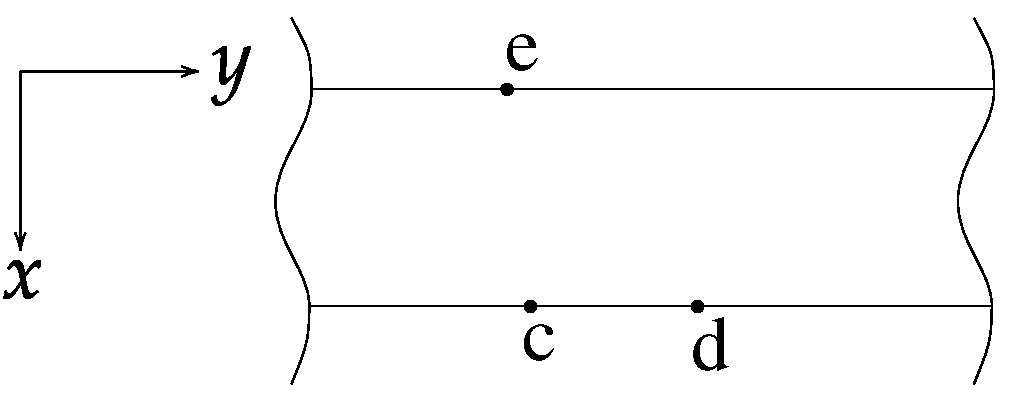
\includegraphics[width=6cm]{fig/fig_4_5_2.pdf}
  \caption{}
\end{wrapfigure}
$V_1 = V_2'$となる磁場中で,この直方体の点c,d,e付近を上から見たときの等電位線を3本,図2に描け\boxnum{8}.

次に,この半導体中を流れる粒子の電荷が負の場合,電圧$V_1$,$V_2'$はどのようになるか.\boxnum{9}に簡潔に述べよ.ただし,電流と磁場の向きは変わらないものとする.
\end{document}

